%
% main.tex
%
% Copyright (C) 2020 by SpaceLab.
%
% DOCUMENTATION-TEMPLATE
%
% This work is licensed under the Creative Commons Attribution-ShareAlike 4.0
% International License. To view a copy of this license,
% visit http://creativecommons.org/licenses/by-sa/4.0/.
%

%
% \brief Main file.
%
% \author Gabriel Mariano Marcelino <gabriel.mm8@gmail.com>
%
% \institution Universidade Federal de Santa Catarina (UFSC)
%
% \version 0.1.0
%
% \date 2020/07/16
%

\documentclass[a4paper,12pt]{book}

\usepackage{spacelab_book}

\title{Documentation Template}
\author{SpaceLab}
\date{\today}

% File metadata
\hypersetup
{
    pdfauthor   = {SpaceLab},
    pdfsubject  = {\thetitle},
    pdftitle    = {\thetitle},
    pdfkeywords = {Nanosatellites, Cubesats}
}

\begin{document}

    \pagenumbering{roman}
    \setcounter{page}{1}

    %
% titlepage.tex
%
% Copyright (C) 2021 by SpaceLab.
%
% Flatsat Platform Documentation
%
% This work is licensed under the Creative Commons Attribution-ShareAlike 4.0
% International License. To view a copy of this license,
% visit http://creativecommons.org/licenses/by-sa/4.0/.
%

%
% \brief Title page.
%
% \author Gabriel Mariano Marcelino <gabriel.marcelino@spacelab.ufsc.br>
%
% \institution Universidade Federal de Santa Catarina (UFSC)
%
% \version 0.2.0
%
% \date 2020/07/16
%

\begin{titlepage}

\thispagestyle{empty}

\begin{flushleft}
SLB-FLATSAT-DOC-v0.2
\end{flushleft}

\vspace{1cm}

\begin{figure}[!ht]
    \begin{flushleft}
        
\includegraphics[width=7cm]{figures/spacelab_logo_full_color_rgb_1000px_72ppi.png}
    \end{flushleft}
\end{figure}

\begin{flushleft}
\Huge{\textbf{\thetitle}}
\rule[0pt]{\textwidth}{5pt}
\end{flushleft}

\vspace{0.2cm}

\begin{flushleft}
\textit{\thetitle} \\
\textit{SpaceLab, Universidade Federal de Santa Catarina, Florianópolis - Brazil}
\end{flushleft}

\vfill
\vfill

\begin{flushright}
June 2021
\end{flushright}

\end{titlepage}

    \cleardoublepage
    %
% authorpage.tex
%
% Copyright (C) 2021 SpaceLab.
%
% Flatsat Platform Documentation
%
% This work is licensed under the Creative Commons Attribution-ShareAlike 4.0
% International License. To view a copy of this license,
% visit http://creativecommons.org/licenses/by-sa/4.0/.
%

%
% \brief Author page.
%
% \author Gabriel Mariano Marcelino <gabriel.marcelino@spacelab.ufsc.br>
%
% \institution Universidade Federal de Santa Catarina (UFSC)
%
% \version 0.1.0
%
% \date 2020/07/16
%

\thispagestyle{empty}

\begin{center}

\textbf{\thetitle}

\textit{January, 2021}

\vspace{1cm}

\textbf{Project Chief:}

Eduardo Augusto Bezerra

\vspace{1cm}

\textbf{Authors:}

Yan Castro de Azeredo \\

\vspace{1cm}

\textbf{Contributing Authors:}

Gabriel Mariano Marcelino \\
André Martins Pio de Mattos \\

\vspace{1cm}


\textbf{Revision Control:}

\end{center}

\begin{table}[!ht]
    \begin{center}
        \begin{tabular}{cL{5cm}L{5.5cm}C{2cm}}
            \toprule[1.5pt]
            \textbf{Version} & \textbf{Author}  & \textbf{Changes}    & \textbf{Date} \\
            \midrule
            0.0     & G. M. Marcelino           & Document creation   & 2020/10/11 \\
            0.1     & Y. C. de Azeredo          & First release       & 2021/01/04 \\
                    &                           &                     &            \\
                    &                           &                     &            \\
            \bottomrule[1.5pt]
        \end{tabular}
    \end{center}
\end{table}

\vfill

\begin{figure}[!h]
	\begin{center}
		
\includegraphics[width=0.25\textwidth]{figures/by-sa.pdf}
	\end{center}
\end{figure}

\textcopyright\  2021 by SpaceLab. \thetitle. This work is licensed under the Creative Commons Attribution-ShareAlike 4.0 International License. To view a copy of this license, visit \href{http://creativecommons.org/licenses/by-sa/4.0/}{http://creativecommons.org/licenses/by-sa/4.0/}.

    \cleardoublepage

    \listoffigures
    \addcontentsline{toc}{chapter}{List of Figures}

    \listoftables
    \addcontentsline{toc}{chapter}{Lista of Tables}

    \printnomenclature
    \addcontentsline{toc}{chapter}{Nomenclature}

    \tableofcontents
    \cleardoublepage
    
    \pagenumbering{arabic}
    \setcounter{page}{1}

    %
% introduction.tex
%
% Copyright (C) 2020 by SpaceLab.
%
% Flatsat Platform Documentation
%
% This work is licensed under the Creative Commons Attribution-ShareAlike 4.0
% International License. To view a copy of this license,
% visit http://creativecommons.org/licenses/by-sa/4.0/.
%

%
% \brief Introduction chapter.
%
% \authors: Gabriel Mariano Marcelino <gabriel.marcelino@spacelab.ufsc.br> and Yan Castro de Azeredo <yan.azeredo@spacelab.ufsc.br>
%
% \institution Universidade Federal de Santa Catarina (UFSC)
%
% \version 0.1.1
%
% \date 2020/07/16
%

\chapter{Introduction} \label{ch:introduction}

The SpaceLab FlatSat Platform is a testbed for CubeSat PCB modules. FlatSats enable easier, faster and a secure method for testing subsystens indenpently while been integrated in a flat design before going to integration on a CubeSat form factor. The PCB can support up to 7 modules, all PC104 pins are interligated to flexibilize its use, only the particularity connection between modules need to be be taken into account. One PC104 has inverted pinout, the board also makes it possible to have two seperate power supplies, a UART to USB converter for four modules, kill-switches activation though SPDTs, Remove Before Flight pin header and a connector for charging batteries. This project is to be used on the GOLDS-UFSC mission \cite{golds-ufsc} during test phase.

\begin{figure}[!ht]
    \begin{center}
        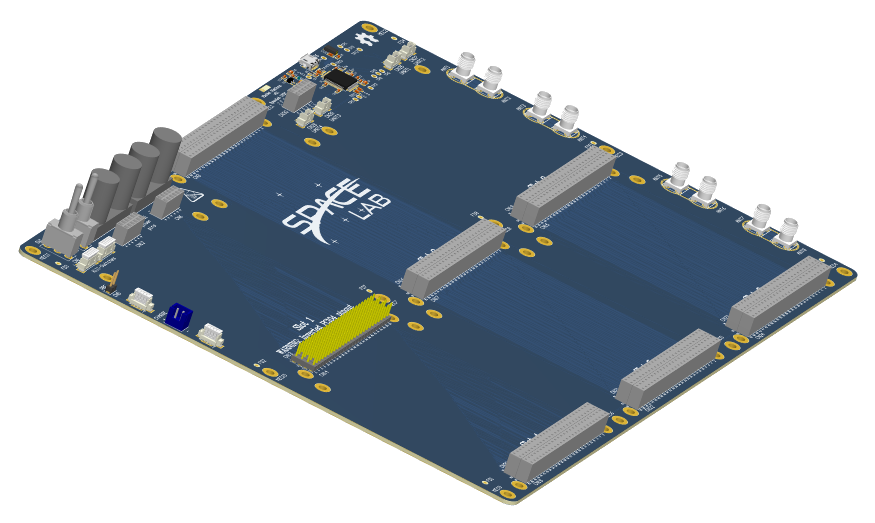
\includegraphics[width=0.75\textwidth]{figures/flatsat_perspective_image.png}
        \caption{3D view of the FlatSat PCB.}
        \label{fig:pcb-3d}
    \end{center}
\end{figure}

All the project, source and documentation files are available freely on a GitHub repository \cite{interface-board-repo} under its respective licenses.
    %
% references.tex
%
% Copyright (C) 2020 by SpaceLab.
%
% Flatsat Platform Documentation
%
% This work is licensed under the Creative Commons Attribution-ShareAlike 4.0
% International License. To view a copy of this license,
% visit http://creativecommons.org/licenses/by-sa/4.0/.
%

%
% \brief References chapter.
%
% \author Gabriel Mariano Marcelino <gabriel.mm8@gmail.com>
%
% \institution Universidade Federal de Santa Catarina (UFSC)
%
% \version 0.1.0
%
% \date 2020/07/16
%

\bibliography{references/test,references/obdh2}

\addcontentsline{toc}{chapter}{References}


\end{document}
